\documentclass[../main/main.tex]{subfiles}

\newdate{date}{29}{10}{2020}


\begin{document}




What is the reason behind this result? Since we know the strong connection between the two theories, now we want to \textbf{derive DBMF from IBMF}
\footnote{We repeat that in annealed networks we are not considering a single network but an average of all the possible random netwrok that you can generate from a degree distribution. Instead, in the quenched network, we take a particular one and we want the result for this specific network.}. \marginpar{ \textbf{Lecture 9.} \\  \displaydate{date}. \\ Compiled:  \today.}
We start from:
\begin{equation*}
  \dot{\rho }_i = - \mu \rho _i + (1 - \rho _i) q_i \qquad \text{ where } \quad q_i = 1- \prod_{j=1}^{N} \qty[ 1 - \beta A_{ij} \rho _j]
\end{equation*}
The Adjacency Matrix is replaced by an \textbf{Annealed Adjacency Matrix} (\textbf{AAM}):
\begin{equation}
  \bar{A}_{ij} = \frac{k_j P(k_i|k_j)}{N P (k_i)}
\end{equation}
which for \emph{random networks} becomes:
\begin{equation*}
  \bar{A}_{ij} = \frac{k_i k_j}{N \expval{k} } = \frac{k_i k_j}{2 L}
\end{equation*}
where the probability  \(  P(k_i|k_j) \) of picking a random node becomes \( k_j \). The last equation reperesent the number of trials that we have to create the connection \( i,j \) over all the possibile connections in the network.
If we substitute the explicit form of the adjiacency matrix in the expression of \( q_i \):
\begin{equation*}
  q_i = 1 - \prod_{j=1}^{N} \qty[1 - \beta \frac{k' P(k'|k)}{N_{k'}} \rho _j]
\end{equation*}
From individual nodes to degree classes:
\begin{equation*}
  \dot{\rho }_k = - \mu \rho _k + (1- \rho _k) \qty[ 1 - \prod_{k'=1}^{N} \qty[1 - \beta \frac{k P(k'|k)}{N_{k'}} \rho _k]^{N_{k'}} ]
\end{equation*}
Assuming \( \beta \rho _k \ll 1 \), we can approximate the product with:
\begin{equation*}
  \dot{\rho }_k = - \mu \rho _k + \beta k (1 - \rho _k) \sum_{k'}^{} P(k'|k) \rho _{k'}
\end{equation*}
and remembering that \( \Theta _k = \sum_{k'}^{} P(k'|k)\rho _{k'}   \):
\begin{equation*}
  \dot{\rho }_k = - \mu \rho _k + \beta k (1- \rho _k) \Theta _k
\end{equation*}
which is the formula obtained for DBMF. Hence, in the DBMF we are implicitly assuming that  \( \beta \rho _k \ll 1 \). This is the reason why DBMF is accurate only around the epidemic threshold. At the end, we are able to pass from IBMF to DBMF and actually we are explaining the difference in the accuracy between the two models.



\subsection{IBMF and Pair approximation}

Let us make a very brief introduction in what it means cut down the chaing to pair approximation.
Until now, all the models that we saw where cutted at the individual level which means that \( \text{Prob} [\sigma _i (t)=0] \) and \( \text{Prob} [\sigma _j (t) = 0] \) are statistically independent:
\begin{equation*}
  \dv{}{t} \rho (i,t) = - \mu \rho (i,t) + \beta \sum_{j}^{} A_{ij} \text{Prob} [\sigma _i(t)=0, \sigma _j(t)=1]
\end{equation*}
Now, if we cut at the link \( (i,j) \) level we have to consider \( \text{Prob} [\sigma _i(t)=0, \sigma _j(t)=1]  \). This involves three nodes terms and so on:
\begin{equation*}
  \dv{}{t} \rho (i,t) = - \mu \rho (i,t) + \beta \sum_{j}^{} A_{ij} \rho (j,t) - \beta \sum_{j}^{} A_{ij} E \qty[X_i (t) X_j (t)]
\end{equation*}
where \(  E \qty[X_i (t) X_j (t)] \) is the two nodes expectation of being infected.
We need an expression for the \( \substack{N \\ 2}  \) equations for \(  E \qty[X_i (t) X_j (t)] \).
The idea is:
\begin{equation}
\begin{split}
  \dv{}{t} E \qty[X_i (t) X_j (t)] &=  - 2 \mu E \qty[X_i (t) X_j (t)] + \beta \sum_{k}^{} A_{ik} E \qty[X_j (t) X_k (t)]  \\
  & + \beta \sum_{k}^{} A_{jk} E \qty[X_i (t) X_k (t)]  - \beta
  \sum_{k}^{} (A_{ik}+A_{jk}) E \qty[X_i (t) X_j (t) X_k (t)]
\end{split}
\end{equation}
and the most common possible closures are:
\begin{equation*}
  E \qty[X_i (t) X_j (t) X_k (t)]   = E \qty[X_i (t) X_j (t)] E[X_k (t)]
\end{equation*}
or
\begin{equation*}
  E \qty[X_i (t) X_j (t) X_k (t)]   = \frac{E \qty[X_i (t) X_j (t)] E[X_j (t) X_k (t)]  }{E[X_j (t)]}
\end{equation*}
where the second is similar to the first but we are considering the two extremes and then the probability that \( j \) is infected.









\chapter{Epidemic spreading on networks: advanced models}

In this chapter, we are gonna study non-Markovian epidemic spreading. In the literature, it is not seen, but if you want to implement a realistic model it is very important.

\section{Markovian Models}

All the models we have seen till now assume that \( \beta  \) (infection process) and \( \mu  \) (recovery process) are constant rates.
This means that movement between compartments takes place at constant rate, or equivalent the probability of jumping from one compartment to another does not depend on the time spent in the compartment. Essentially, we are considering a memoryless process.
The jump are memoryless, i.e. we are running a Markov chain.

The fundamental property of a Markov chain is called \textbf{Markov property}: \emph{the jump probability at time \( t + \Delta t \) does not depend on elapsed time, but only on \( t \)}, i.e. we have not to take into account the time that we spent in that compartment.
This property is very useful for mathematical treatments.

Jumps made at a constant rate (\( \beta  \) and \( \mu  \)) imply that the time spent inside each compartment \( \tau  \) follows a expoential distribution:
\begin{equation}
  P(x) = \tau e^{- \tau x}
\end{equation}
with mean \( \tau = \frac{1}{\mu }\), i.e. \( \tau  \) is the infectious period (average time spent in \( I \)).

What are the implication of this property? The most important one is that an exponentially distributed infectious period implies that the most probable duration of the disease is 0. Indeed, the probability decreases with time.
More particularly, it depends on the mean, but in any case the most probable jump (time in which I am making the jump) is at the beginning.
It is something that is not realistic, indeed if you got influenza at least you will spend some time infected.
And actually, if you are looking how infectius period are distributed in real life, it is something which is quite different. For a disease, you know exactly when it starts but do not you know when it ends.
For instance, let us consider the left plot in Fig. \ref{fig:09_1} for 2009 H1N1 Influenza. For this type of diesease the plot show the distribtuion of the infectious period, which has as probable value 2 days and an half. The most important things is that it is not 0. On the right, we have also the estimates for Covid-19. One process we use to measure the infectious period is the \textbf{serial interval}, i.e. from symptoms to symptom. Or we have also the \textbf{generation time}, i.e. from infection to infection. Obviously, these are approximations but can give you some means.

\begin{figure}[h!]
\begin{minipage}[c]{0.5\linewidth}
\centering
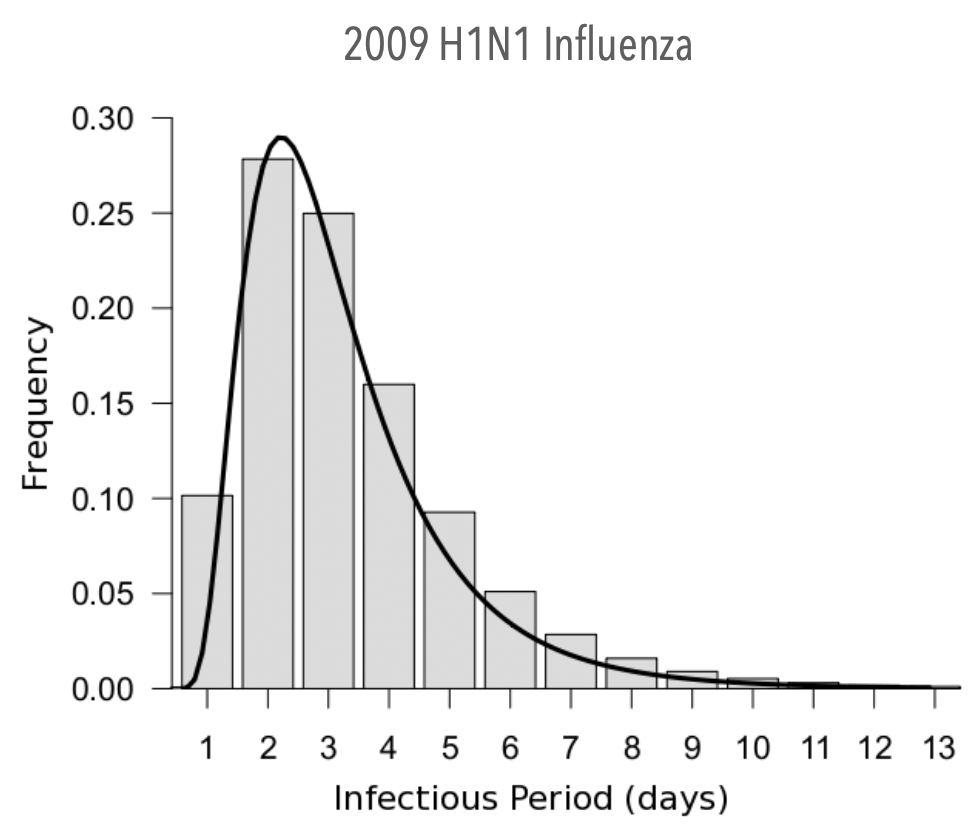
\includegraphics[width=1\textwidth]{../lessons/image/09/1.png}
\end{minipage}
\begin{minipage}[]{0.5\linewidth}
\centering
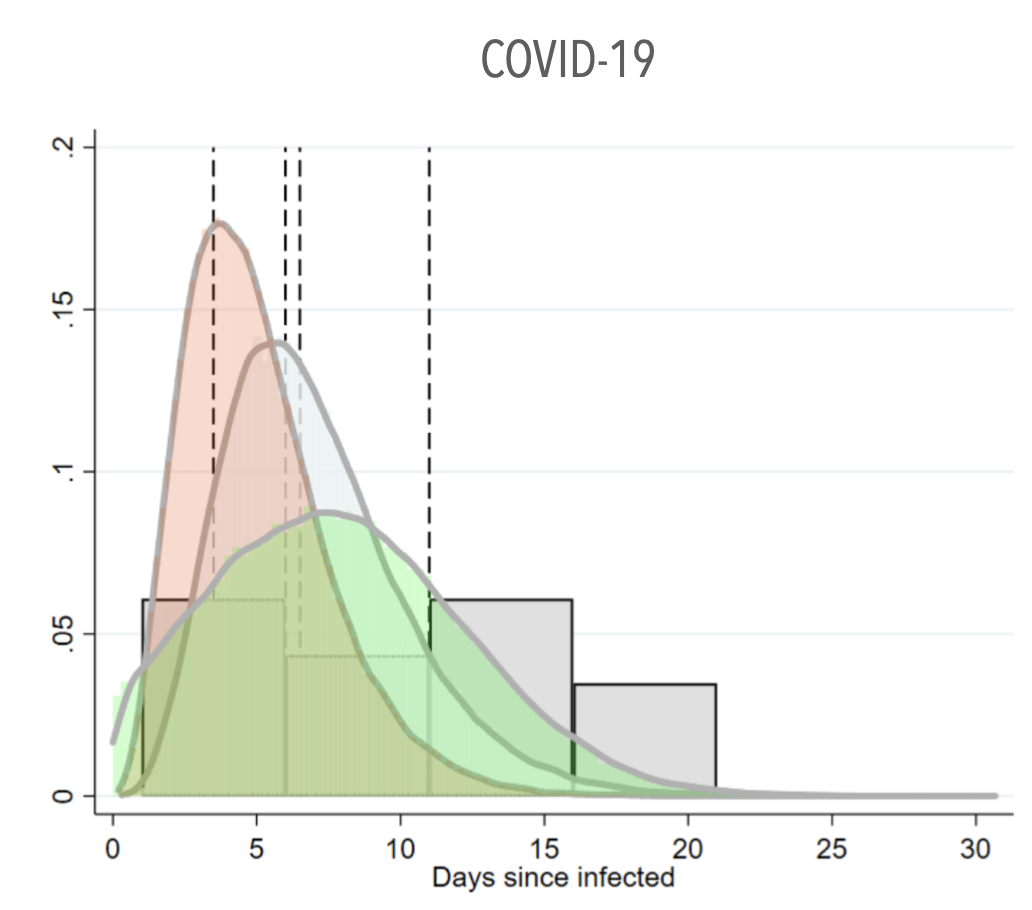
\includegraphics[width=1\textwidth]{../lessons/image/09/2.png}
\end{minipage}
\caption{\label{fig:09_1} \textbf{Left:} Histogram of 1009 H1N1 Influenza. \textbf{Right:} distribution  of Covid-19. }
\end{figure}

The problem is that, all these results demonstrate that these kind of diseases are non-markovian: transition probability depends on the time spent in a compartment. Indeed, patients usually spend some time infected before starting to recover.




\section{Non-Markovian Epidemic Spreading}

How are we gonna model this non markovianity?
What are the distribution that better describe what we saw in the data?

Patients usually spend some time infected before starting to recover. This situation is better approximated by a \textbf{Gamma distribution}:
\begin{equation}
  P(x) = \frac{1}{\Gamma (k) \theta ^k} x^{k-1} e^{- \frac{x}{\theta }}
\end{equation}
where \( k \) is the \emph{shape}, \( \theta  \) the \emph{scale} and   \( \Gamma (x) \) is the \emph{gamma function}:
\begin{equation*}
  \Gamma (x) = \int_{0}^{\infty } t^{x-1} e^{-t} \dd[]{t}
\end{equation*}
The gamma distribution has mean \( k \theta  \) and variance \( k \theta ^2 \).
This shape start to be somehow what we saw in the data.

What is similar to the gamma distribution is the \textbf{Erlang distribution}, where we have the factorial instead of the Gamma function:
\begin{equation}
  P (x) = \frac{\lambda ^k x^{k-1}e^{- \lambda x} }{(k-1)!}
\end{equation}
or the \textbf{Weibull distribution}:
  \begin{equation}
  P(x) =
    \begin{cases}
     \frac{k}{\lambda } \qty(\frac{x}{\lambda })^{k-1} e^{- (x/\lambda )^k} & < \ge 0  \\
    0 & x <0
    \end{cases}
  \end{equation}
All of these distribution are able to reproduce real histograms.

However, the question still remains: how to include non-markovian elements in classical epidemiological models (with the assumption of markovian...)?
We use a trick for the indectious period: \emph{the sum of exponential random variables obeys a Gamma distribution}.
How we are gonna incorporate that in our model? Instead of having just one transition at a coastant rate (expoential distribution), what we need to have to have a gamma distribution?


The trick is the fact that instead of having just one transition, we are gonna include more and more transitions. Instead of having just one single infectious state, individuals move from one  compartment to the other, such that they spend at least some time infectious before starting the recovery. We obtain again a Markovian model.

\subsection{SIR Model with Multiple Infectious Stages}

To repeat, the solution is using \textbf{multiple infectious compartment}, i.e. SIR in well mixed populations becomes \( S I_1 I_2 \dots I_k R \). For instance, we are imposing that these transitions are sequential:
\begin{equation}
\begin{split}
  S + I & \overset{\beta }{\rightarrow } I + I_1   \\
  I_1 & \overset{K \mu  }{\rightarrow } I_2 \\
   I_2 & \overset{K \mu  }{\rightarrow } I_3 \\
   & \vdots \\
   I_k & \overset{K \mu  }{\rightarrow } R
\end{split}
\end{equation}
Hence, if I want to get recovered I need to spent some times infectious, but the model is still markovian! More precisely, the equations are:
\begin{equation}
\begin{split}
  \dv{s}{t} &= - \beta s i  \\
  \dv{i_1}{t} &= \beta s i - K \mu i_1 \\
  \dv{i_2}{t} &= K \mu i_1 - K \mu i_2 \\
  &\vdots \\
  \dv{r}{t} &= K \mu i_k
\end{split}
\end{equation}
where the rate of each \( I \) transition is \( K \mu  \) and with \( i = \sum_{k=1}^{K} i_k   \).
We got that this is the infectious period distribution:
\begin{equation}
  P(\tau ) = \frac{(\mu K)^K}{\Gamma (K)} \tau ^{K-1} e^{- \mu K \tau }
\end{equation}
where the mean is still \( 1/ \mu  \), but the shape is totally different.
which is the gamma function.
We have two special cases:
\begin{itemize}
\item if \( K=1 \), we obtain an exponential distribution;
\item if \( K \rightarrow \infty  \) fixed, we obtain a delta distribution.
\end{itemize}

Other quantities are:
\begin{equation*}
  R_0 = \frac{\beta }{\mu }
\end{equation*}
and the \textbf{final epidemic size}:
\begin{equation*}
  r_ \infty  = 1 - e^{- R_0 r_ \infty }
\end{equation*}
Moreover, we have an early growth:
\begin{equation*}
  i(t) \simeq i_0 e^{\lambda t}
\end{equation*}
instead of \( i(t) \simeq i_0 e^{(\beta - \mu )t}  \). Hence, the disease is growing faster and has a shorter duration.

With \( \lambda  \) as the solution of:
\begin{equation*}
  R_0 = \frac{\lambda }{\mu  \qty(1- \qty(\frac{\lambda }{K \mu } + 1) ^{-K}) }
\end{equation*}

The \( S I_1 I_2 \dots I_k R \) model has several limitaionts:
\begin{itemize}
\item it is defined only for well-midex populations;
\item focus only on the infectious period distribution. We have that infections are still Markovian and this model only reproduces as Gamma distribution.
\end{itemize}


\subsection{Generalized SIS Model}

Now, we are going to present something which is more general where we can include non-markovian both in recovery and infections.
Is it possible to write down a general model on networks? The answer is  yes, it is a bit more complicated and we still needs some kind of approximation at some point.
In particular, we need a mean-field approximation.

We have to change our point of view. We are gonna use a slightly different approach, i.e. instead of probabilities we are gonna talk about events. The idea is that we are gonna modelling in this case the infections and recoveries with two random numbers which we extract from distribution and are as general as possible.

The ingredients are:
\begin{itemize}
\item a random number \( R_i (t) \): recovery time of node \( i \) when infected;
\item a random number \( M_{ij} (t) \): infection times at which node \( i \) tries to infect node \( j \).
\end{itemize}
In order:
\begin{itemize}
\item node \( i \) get the infection at time \( t \);
\item we extract the random number \( R_i (t) \) which represents the time in which node \( i \) is gonna recovery (or, the time for which it stay infected);
\item then, we extract the random number  \( M_{ij} (t) \) which reprsenets the number of trials that \( i \) try to infect node \( j \) while infected;
\item we generate a sequence of times
\begin{equation*}
  T_{ij}^{(1)} \le \dots \le T_{ij}^{(M_{ij}(t))} \le R_i (t)
\end{equation*}
in which node \( i \) try to infect node \( j \). For instance, \(  T_{ij}^{(1)} \) is the first time that node \( i \) try to infect node \( j \) then we have the second time and so on;
\item I am gonna repeat the last step for all my neighbours.
\end{itemize}
Hence, the trasmitibility of the diesease is seen as how many trials I am gonna make to infect.
One important thins is that \( R_i (t) \) and \( M_{ij} (t) \) can be drawn from any distribution and not only from the exponential one.
How do we extract the \( T_{ij} \) is not important at this point, because we are only gonna focus on the distribution of \( R_i (t) \) and \( M_{ij} (t) \).


Now, let us make some assumptions to make the model more reasonable and then treat it analytically. We assume that:
\begin{itemize}
\item \( R_i (t) \) and \( M_{ij} (t) \) do not depend on time, i.e. \( R_i (t) \equiv R_i \) and \( M_{ij} (t)  \equiv M_{ij} \);
\item \( R_i (t) \) and \( M_{ij} (t) \)  do not depend on \( i \) and \( j \), i.e. same distribution for all the nodes \( R_i \equiv R \) and \( M_{ij} \equiv M \).
\end{itemize}
hence, we are assuming that these numbers should not depend on time and for instance they are typical for the disease. It is valid both for the recovery and for the infections. However, if we consider restrictions as lockdown and so on these number should change, but for the let us consider the simplest model without such restrictions. Indeed, with these assumptions we are reducing the complexity.

We call:
\begin{itemize}
\item \( E[R] \), the expected value of \( R \);
\item \( E[M] \), the expected value of \( M \);
\item \( v_i \), the probability that node \( i \) is infected in the steady state.
\end{itemize}



Now, let us build the model:
\begin{enumerate}
\item let us suppose that we are in the steady state of the system (all the transient are passed).
In a large time interval \( [0,S] \) the number of times node \( j \) has been infected is proportional to \( S \) (it is linear).
Since the length of each infected period is \( E[R] \), the \textbf{number of infected periods} experienced by a node \( j \) (number of times a node has been infected in the interval \( [0,S] \)) can be written as:
\begin{equation*}
  \frac{v_j S}{E[R]}
\end{equation*}

\item during each infected period, node \( j \) will try to infect \( i \) an average \( E[M] \) number of times. So, the \textbf{total number of infection attempts} from node \( j \) to \( i \) in a large period of time are:
\begin{equation*}
  \frac{v_j S E[M]}{E[R]}
\end{equation*}
the number of times \( j \) has been infectious multiplied by the number of infection attempts per each time;

\item then, we make the \textbf{mean-field assumption}: the  conjunct probability that $j$ is infected and $i$ is susceptible is:
\begin{equation*}
  \text{Prob} [ \sigma _i (t)=0, \sigma _j (t)=1] \rightarrow \underbrace{\text{Prob} [\sigma _i (t) = 0]}_{(1-v_i)} \underbrace{\text{Prob} [\sigma _j (t) = 1]}_{v_j}
\end{equation*}

\item we can write the \textbf{total number of successful infection attempts} for \( j \) to \( i \) as:
\begin{equation*}
  S \frac{E[M]}{E[R] } v_j (1-v_i)
\end{equation*}
that is the total number of attempts multiplied by the probability that $i$ was not infected.

Summing over all the neighbors of $i$ we have the the \textbf{total number of successful infections} \( i \) will receive during interval \( [0,S] \) is:
\begin{equation*}
  S \sum_{j=1}^{N}  a_{ij} \frac{E[M]}{E[R]} v_{j} (1-v_i)
\end{equation*}

\item in the \emph{steady state} the number of successful infections (\(  S \sum_{j=1}^{N}  a_{ij} \frac{E[M]}{E[R]} v_{j} (1-v_i) \)) is asymptotically equal to the number of infected periods experienced by \( i \): \( v_i S / E[R] \). Thus we have:
\begin{equation}
  \cancel{S} \sum_{j=1}^{N}  a_{ij} \frac{E[M]}{\cancel{E[R]}} v_{j} (1-v_i) = v_i \frac{\cancel{ S}}{\cancel{E[R]}} \qquad \rightarrow \qquad  v_i = E[M] (1- v_i) \sum_{j=1}^{N} a_{ij} v_j
\end{equation}
hence the probability of \( i \) being infected depends by the sum over all its neighbours, times the term \( E[M] \) which is the average infection attempts that it is gonna experience during the evolution.
\end{enumerate}

Do the last expression sound familiar? This is exactly the same expression of the IBMF but with a generic infection term \( E[M] \):
\begin{equation*}
  \mu \varepsilon _i^* = \beta ( 1 - \varepsilon _i^*) \sum_{j=1}^{N} a_{ij} \varepsilon _j^*
\end{equation*}

The implications are:
\begin{itemize}
\item the definition of \( M \) implicitly includes the recovery term: \( T_{ij}^{(1)} \le \dots \le T_{ij}^{(M_{ij}(t))} \le \mathcolorbox{green!20}{R_i (t)} \);
\item exponential case: \( E[M] \) is the expected number of infection events in a Poisson preocess with intensity \( \beta  \) within an exponential recovery time with expectation \( 1/ \mu  \). Thus: \( E[M] = \beta / \mu  \).
\item epidemic treshold (lower bound):
\begin{equation*}
  m_c = E[M_c] = \frac{1}{\Lambda _{max}}
\end{equation*}
\end{itemize}
Hence, this is the form in which we can generate a generic model from. 










\end{document}
